\chapter{Introduction}

This document is a portfolio for CS4157, Software Quality, taught by Dr. Ita Richardson. It aims to illustrate and summarise the key concepts explored, and the learning process, within the module. Each week will be a briefly summary of the key points that I took from the lectures, and a discussion on any papers, and how useful, or useless, I found them. Summaries of meetings held by the group tasked with the module project will also be listed. 

\chapter{Week 1}
\section{Learnings}

The three key things I took from this weeks lecture were:

\begin{enumerate}
\item Eliminate testing by refining process
\begin{itemize}
\item By following a quality process and focusing on quality throughout, the need for testing can be reduced.
\end{itemize}
\item Other things in software system
\begin{itemize}
\item Be ware of other items in the software system: hardware, users, environment etc
\end{itemize}
\item Problem based learning
\begin{itemize}
\item Tackle the issue and learn how to solve the problem by working on the problem
\end{itemize}
\end{enumerate}

\section{Paper}

The paper that was looked at this week was "Understanding the implementation of software process improvement innovations in software organisations" \parencite{week1}. The goal of the paper is to "achieve a better understanding of the processes influencing the introduction, organizational implementation and adoption of software process improvement innovations in and by software companies" \parencite{week1}.

I found the paper a bit difficult to read, as it focused on a number of research methodologies that I am not familiar with, but I did like the breakdown on types of innovation.

\textbf{Individualistic Perspective} assumes that single individuals  that the main source of innovation within an organisational structure. Actions by these people are "not seen to be constrained by external factors" \parencite{week1}. These individuals are self guiding, and focused, and any decisions they make are made in order to "maximise value or utility" \parencite{week1}

\textbf{Structuralist Perspective} assumes that "innovation is determined by objectively existing organizational characteristics" \parencite{week1}. This view seems to place the chance of innovation on factors within the organisation, such as an "organisations size, its task structure differentiation, its task complexity, its employees job specialization and their professionalism" \parencite{week1}.	 

\textbf{Interactive Process Perspective} assumes innovation is "dynamic, continuous phenomenon of change over time" that is a result of both individual and organisational factors \parencite{week1}. It focuses on the interactions between individual and organisations. Innovation is the result of the "continuous interaction of the actions of individuals, structural influences and innovation itself" \parencite{week1}.

\section{Meeting}

No meeting held this week.

\chapter{Week 2}

\section{Learnings}

\begin{enumerate}
\item Quality priority depends on perspective
\begin{itemize}
\item I defined quality as the amount of reliability that a product or service has
\end{itemize}
\item When is it really important to ensure high quality?
\begin{itemize}
\item The output, where it is being used? - Example: salt from fast food dissolved seat belts. All possibilities cannot be tested for!
\end{itemize}
\item 'Good Enough' software - for the purpose it is built for
\begin{itemize}
\item Functions are right, the cycle time is right, the quality is right, development productivity is right - capability of process.
\end{itemize}
\end{enumerate}

\section{Paper}

This weeks paper was "Evaluation of Connected Health Technology" \parencite{week2}. It noted that many people who develop connected health solutions (CHS) "are not from a primarily health technology related background" \parencite{week2}. They tend to originate from engineering and IT disciplines, as well as the mobile technology and sensor sectors. This paper showed the range of knowledge needed to correctly evaluate a CHS. 
\begin{itemize}
\item Knowledge of research governance and ethics
\item Project management
\item Statistical knowledge
\item Technology knowledge
\item Clinical experience
\item Design and implementation of pre and post evaluation questionnaires
\item Regulatory knowledge
\item Procurement of consumables or technology.
\item \parencite{week2}
\end{itemize}	

I also spoke with a psychiatric nurse about connected health briefly, and her thoughts are summarised below: 

\textbf{Can you think of anything in your line of work that would benefit from a system link this, a condition that requires 24 hour monitoring but the nursing levels couldn't support that level of monitoring?}

\textit{We actually have something like this in work already it wouldn't be as advanced as the YouTube clip but it's along the same lines. It's in some houses at night where there aren't staff and if it detects movement it alarms and a staff member goes to the house,there's motion detectors around the house, I don't fully agree with them because in our case in work they're using them in houses where there are people with epilepsy and they may have silent seizures which the technology isn't going to pick up maybe if it was more advanced it might but it's not at that level at the moment so there's high risks being taken to save money on staff. }


\section{Meeting}

\textbf{Date}: Feb 6th\newline
\textbf{Attendees}: Chris, Cian, Shane\newline
\textbf{Absent}: Brian\newline
\textbf{Notetaker}: Cian\newline
\textbf{Chairperson}: Chris\newline \newline
\textbf{Actions for Next Week}
\begin{enumerate}
\item Each person to find and summarise a paper relating to Connected Health
\item Set up a Google Doc which contains a section for each of the following:
\begin{itemize}
\item Documents Read
\item Meeting Minutes
\item Main Software Quality Plan Document
\end{itemize} 
\item Find a working example of a Software Quality Plan
\item Make sure all members can access the UL Library
\item Chris to talk to a Psychiatric Nurse regarding the project
\item Research existing products
\item Type up the meeting minutes document
\end{enumerate}

\textbf{Brainstorming on domain for CH}
\begin{itemize}
\item Alzheimers - Virtual Fencing
\item People on Clinical Trials - Monitor changes
\item Blind / Deaf People - System to notify them of things they can't notice
\item Morbidly Obese People - Monitor bed sores etc
\item Air Monitoring - Cleanliness, humidity
\item Sleep Apnea - System to wake sufferers of this ailment.
\end{itemize}

\textbf{General System Ideas}\newline \newline
Store information regarding the changes in medication and compare that to the changes in the person.
\chapter{Week 3}

\section{Learnings}
\begin{enumerate}
\item Project Capability
\begin{itemize}
\item How good is the project, and the company who make it?
\end{itemize}
\item Project Maturity
\begin{itemize}
\item The maturity of the company - new, start up, experience etc.
\end{itemize}
\item Total Quality Management
\begin{itemize}
\item Collection of processes to achieve quality
\end{itemize}
\end{enumerate}

\section{Paper}

The paper reviewed this week was "Assessing the Impact of Continuous Quality Improvement/Total Quality Management: Concept versus Implementation" \parencite{tqm}. This paper discussed the outcomes on a sample of hospitals using TQM processes, and "focuses on factors influencing the implementation of quality improvement activities and the perceived impact on human resources development, patient care outcomes, and financial outcomes" \parencite{tqm}. The goal was that to use of TQM tools would "result in an ability to both maintain and improve quality while controlling increases in costs" \parencite{tqm}. While this is an older paper, an interesting statistic that was highlighted was that the majority of sampled with "69 percent actively begun to implement the basic components of TQM" \parencite{tqm}.

An interesting point was the use of employee empowerment and involvement to drive the TQM process. The division of the culture within a organisation into four areas was also interesting, but was based on a considerable amount of other papers that I felt were outside the scope of this module, and were based on \parencite{quinn}. 

\begin{enumerate}
\item Group Culture - Based on "norms and values associated with affiliation, teamwork, and participation" \parencite{tqm}
\item Development Culture - Based "on risk taking innovation and change" \parencite{tqm}
\item Hierarchical Culture - Based on "reflecting the norms and values associated with bureaucracy" \parencite{tqm}
\item Rational Culture - A culture based on "emphasizing efficiency and achievement"\parencite{tqm}
\end{enumerate}

The paper got a bit heavier in terms of analysis after this and it was a bit difficult to follow without having the experience and domain knowledge needed to perform a similar study.

\section{Meeting}
\textbf{Date}: Feb 13th\newline
\textbf{Attendees}: Chris, Cian, Shane\newline
\textbf{Absent}: Brian\newline
\textbf{Notetaker}: Shane\newline
\textbf{Chairperson}: Cian\newline \newline
\textbf{Feedback from Ita} \newline \newline
Feedback from nurse was useful and in the right direction for the kind of risks we should be thinking about.

Our Plan needs to be able to detect the problems that could occur.


\textbf{Risks/Patient Safety}
\begin{enumerate}
\item Focusing too much on interoperability, not enough on client safety
\item Conflict of laws between countries, acceptance criterias differ
\item Data representation
\begin{itemize}
\item What is the recommended/normal amount of times people wake at night
\end{itemize} 
\item Misconfiguration of system
\item Misuse (Malicious or otherwise) of both information and the system.
\item Ease of use, Domain knowledge
\item Reimbursement, doctors need to be paid.
\item Reliability of internet, bandwidth and connectivity.
\item Confidentiality/Invasiveness
\item Encryption/Security
\item Guidelines for diagnosis
\item Attach patients to people under NDA.
\item Four Threats
\begin{itemize}
\item Confidentiality
\item Integrity
\item Availability
\item Quality of the software quality plan
\end{itemize}
\item The main point is to improve patient outcome.
\end{enumerate}

\textbf{Actions}
\begin{itemize}
\item Chris - look into ethical Approval
\item Web of science, each reading a paper - with a view towards risk.
\item Research ethics
\end{itemize}

\chapter{Week 4}

\section{Learnings}
\begin{enumerate}
\item Improved process leads to improved product
\begin{itemize}
\item Improved manufacturing process leads to improved product. Why not the same with software?
\end{itemize}
\item Regulations for software
\begin{itemize}
\item FDA in America, EU directives within the EU.
\end{itemize}
\end{enumerate}

\section{Paper}

The paper looked at this week was "The influence of EU law on the social character of health care systems in the European Union"  \parencite{week3}, specifically Chapter 5 pertaining to medical devices. 

The paper concerned the way that the EU controlled the regulation of medical devices, and how it is changing. It spoke of how deregulation is occuring at a national level, with decisions regarding medical devices being made as a whole. This is an attempt to "harmonise and standardize" medical devices across the Community \parencite{week3}. Discussion of the learnings are in section~\ref{sec:medicald}.

\section{Meeting}

\textbf{Date}: Feb 20th\newline
\textbf{Attendees}: Chris, Cian, Shane, Brian\newline
\textbf{Notetaker}: Chris\newline
\textbf{Chairperson}: Brian\newline \newline

\textbf{Identify one aspect of a software quality plan}
\begin{enumerate}
\item Risk Management and Identification
\item Data Privacy 
\item Staff Training
\item Actual Users of the system
\item Software and Hardware
\item System Usage
\item Device Classifications (C1, C2, C3)
\item Different Knowledge bases (eg doctor, nurse, carer, soft engineer)
\item Location/Environment (home vs hospital, small vs large) - CIAN
\item Ethical Approval
\item Legal Issues
\end{enumerate}

\textbf{Examples}
\begin{itemize}
\item Hardware: how to deal with repairs? Severity (monitor vs server)
\item Software: How easy to fix on the spot? How easy to get back up and running if it falls down?
\item Identity risks, manage risks, prevent risks, level of risk
\item Adherence to regulations
\item Testing controls
\end{itemize}

\textbf{Actions}
\begin{itemize}
\item 1000 words on selected topic
\item Data Privacy - Brian
\item Software and Hardware - Shane
\item Device Classification - Chris
\item Location and Environment - Cian
\end{itemize}

\section{Device Classification Assignment}
\label{sec:medicald}

One aspect that needs to be considered as part of any software quality plan is the type of medical devices being used, and their use within the connected health system. It is important that any devices used within a connected health system adhere to guidelines set out in MEDDEV 2.4/1 Rev. 9. These guidelines help to govern the quality of devices used for medical reasons, and if a device is unclassified, then it would lead to more work in the setup of the system to ensure that said device is safe for use within a medical setting. The European Union requirements for classification of medical devices are set out in Annex IX of the Council Directive 93/42/EEC, while the Food and Drug Administration (FDA) is responsible for this in the United State. In Canada, the Medical Devices Bureau of Health Canada is responsible, while section 41BD of the Therapeutic Goods Act 1989 and Regulation 3.2 of the Therapeutic Goods Regulations 2002 outlines the usage of such devices in Australia, and is under the control of the Therapeutic Goods Administration. It is important that when designing a connected health solution that you are cognisant of the classification of each device, especially if you wish to use the solution in multiple jurisdictions. 

Devices are categorised based of what risk is attached to its usage. Class I is a low risk device, Class II is medium risk, Class IIb is higher risk and Class III is highest risk. There are a number of rules which aid the classification of a device. Rules 1 through 4 identify a non-invasive device. An example of this would be a hearing aid. Rules 5 to 8 refer to invasive devices, which is any device intended, by the manufacturer, to be used, in whole or part, to penetrate the body of a human being through a body orifice or through the surface of the body. A key example of this would be an injection. Rules 9-12 cover what are called Active Devices. These refer to devices that are active and implantable. A pacemaker would be an example of an active device. Rules 13 through 18 are special rules. These deal with devices that cover a range of possibilities

\begin{itemize}
\item Devices incorporating integral medicinal substances liable to act in an ancillary way on the human body
\item Devices used for contraception or prevention of STDs.
\item Devices for disinfecting medical devices
\item Devices for recording X-Ray diagnostic images
\item Devices using non-viable animal tissues or derivatives
\item Blood bags
\end{itemize}

In relation to these devices, a plan needs to be established on how to deal with their handling, storage, disposal, and any training that may be needed by the user, or given to the user. An obvious example is any situation dealing with bladder problems – the patient may have a drainage bag and catheter. There would need to be awareness of how to correctly prepare these devices on a patient, and to ensure their proper installation, usage and disposal, and any lack of attention to these areas would lead to high risk of infection. In terms of developing a quality plan for a connected health system, it’s vitally important that these issues are part of any plan. While the how and why of the classification of devices is not an issue within the scope of the plan, how to deal with, manage, and use these devices is very much an issue that needs to be addressed. The range of devices will differ greatly depending on the connected health system, the environment of the system and even on a patient to patient basis, so in this situation, it is important to break down the system to granular devices and ensure compliance.

\chapter{Week 5}

\section{Learnings}
\begin{enumerate}
\item Business importance of software increasing
\begin{itemize}
\item 90\% of the cost of a car is software
\end{itemize}
\item Business Benefits
\begin{itemize}
\item Return on investment increases, productivity increases, overall effect decrease. More money, less work with a good process.
\end{itemize}
\item Software Process Improvement
\begin{itemize}
\item Productivity up, Defects down, Error Rates down, Costs down, On Time Deliverables up, Rework down and savings in test time. 
\end{itemize}
\item Software Process Models
\begin{itemize}
\item Capability Maturity Model, ISO 15504, Configuration Management, Assessment of System
\end{itemize}
\end{enumerate}

\section{Paper}

\section{Meeting}

This weeks meeting focused on the presentation of current findings for the Software Quality plan and paper.

\textbf{Date}: Feb 20th\newline
\textbf{Attendees}: Chris, Cian, Shane, Brian\newline
\textbf{Notetaker}: Cian\newline
\textbf{Chairperson}: Shane\newline \newline

\textbf{What is your presentation content?}
\begin{enumerate}
\item Dealing with classified devices
\begin{itemize}
\item CMMI
\item FDA
\item Differences
\end{itemize}
\item Data Privacy Issues
\begin{itemize}
\item Network Security
\end{itemize}
\item Environmental Effects
\begin{itemize}
\item Location
\item Installation
\item When things break, and the impact that has on the system
\end{itemize}
\item Hardware and Software Issues
\item Crisis Management
\begin{itemize}
\item Automation
\item Who to call?
\end{itemize}
\end{enumerate}

\textbf{Recap: What have we covered?}
\begin{itemize}
\item Hardware and Software - make more generic.
\item Location and Environment
\item Data Privacy
\item Classification of Medical Devices
\begin{itemize}
\item Regulations for these devices
\item Handling of devices
\item Storage of devices
\item Disposal of devices
\item Training
\end{itemize}
\item Microsoft Excel as a Medical Device?
\begin{itemize}
\item Used by Doctors
\item Cognisance of the intention of use
\item Burden of proof on company to prove fit for purpose.
\end{itemize}
\end{itemize}

\textbf{Actions}
\begin{itemize}
\item Brian - Ethical Approach
\item Presentation - 5 slides each on topic from last weeks meeting
\item Presentation Practice on Monday and Wednesday
\item Time keeping - ensure under 20 minutes total
\end{itemize}


\chapter{Week 6}

\section{Learnings}

This week was the preparation and practice of presentations in relation to the Software Quality plan being devised for this module. A 20 minute presentation was created with each team member taking 5 minutes on their chosen topic. 

\section{Paper}

No paper read this week due to presentation practice and preparation. Previous weeks paper used to guide this.

\section{Meeting}

This weeks meeting focused on preparing the presentation content and practising.

\textbf{Date}: Feb 26th\newline
\textbf{Attendees}: Chris, Cian, Shane, Brian\newline
\textbf{Notetaker}: Brian\newline
\textbf{Chairperson}: Shane\newline \newline

Order of the presentation
\begin{enumerate}
\item Shane - Hardware and Software
\item Cian - Environmental Factors
\item Brian - Data Privacy
\item Chris - Medical Devices
\end{enumerate}

Other tasks were

\begin{itemize}
\item Merge Slides
\item Create intro slide
\item Create conclusion slide covering other topics not covered yet
\item Cian wanted to dance, but it was vetoed
\end{itemize}

\chapter{Week 7}

\section{Learnings}

Q\&A Session on 14/04

\begin{itemize}

\item How to deal with risk?
\begin{itemize}
\item Matrix used by NASA to assess risk in an environment
\item What's the worst case?
\item How likely is this to happen?
\end{itemize}

\item How to manage stakeholders?
\begin{itemize}
\item There should be one champion in a hospital to help lower stakeholder conflict.
\end{itemize}

\item Privacy Issues
\begin{itemize}
\item Password sharing
\item Sharing ID cards
\item Not logging out
\item Multiple logins to deal with one patient (Usability Vs Privacy concerns)
\end{itemize}

\end{itemize}

HIQA - Hospital Information Quality Assurance

Concept of two level password - Second one is full access, but usage is logged with meeting called on use to establish the reason for its use, and if it was valid.

\section{Paper}

Focus on CH talk and questioning this week

\section{Meeting}

None this week

\section{Question Prep}
\begin{enumerate}
\item How difficult is it to integrate a connected health solution with an existing system?
\item Failures in connected health system? How are failures handled? Repercussions?
\item Integration of IT and Healthcare - What usability issues arise and how are they handled?
\end{enumerate}

\chapter{CH Talk and Q\&A}

The CH talk on 13/03 highlighted a number of areas of interest.

\begin{itemize}
\item Connected Stakeholders
\begin{itemize}
\item All stakeholders are involved in the solution together. Each has a different knowledge area and expertise to bring to the system in order to make it work. Different disciplines of two presenters an example
\end{itemize}
\item Empower the patient to be able to look after themselves. @home
\item Evidence based standards - replace existing healthcare models
\item Need to support deployment, adaptation and reimbursement.
\item Need to illustrate the savings, to time, money and personnel, of a Connected Health Solution.
\item Danger of siloed information
\end{itemize}

There were a number of challenges highlighted

\begin{enumerate}
\item Fragmented Systems
\item No fixed pathways for CHS
\item Importing existing information
\begin{itemize}
\item E-Health Records
\item CDROM and physical files
\end{itemize}
\item Lack of information provisioning carers
\end{enumerate}

CH Deployment needs to be concerned with usability and acceptability. The \textit{Delone and McLean} model for quality deployment utilised.
\chapter{Week 8}

\section{Learnings}
\begin{center}
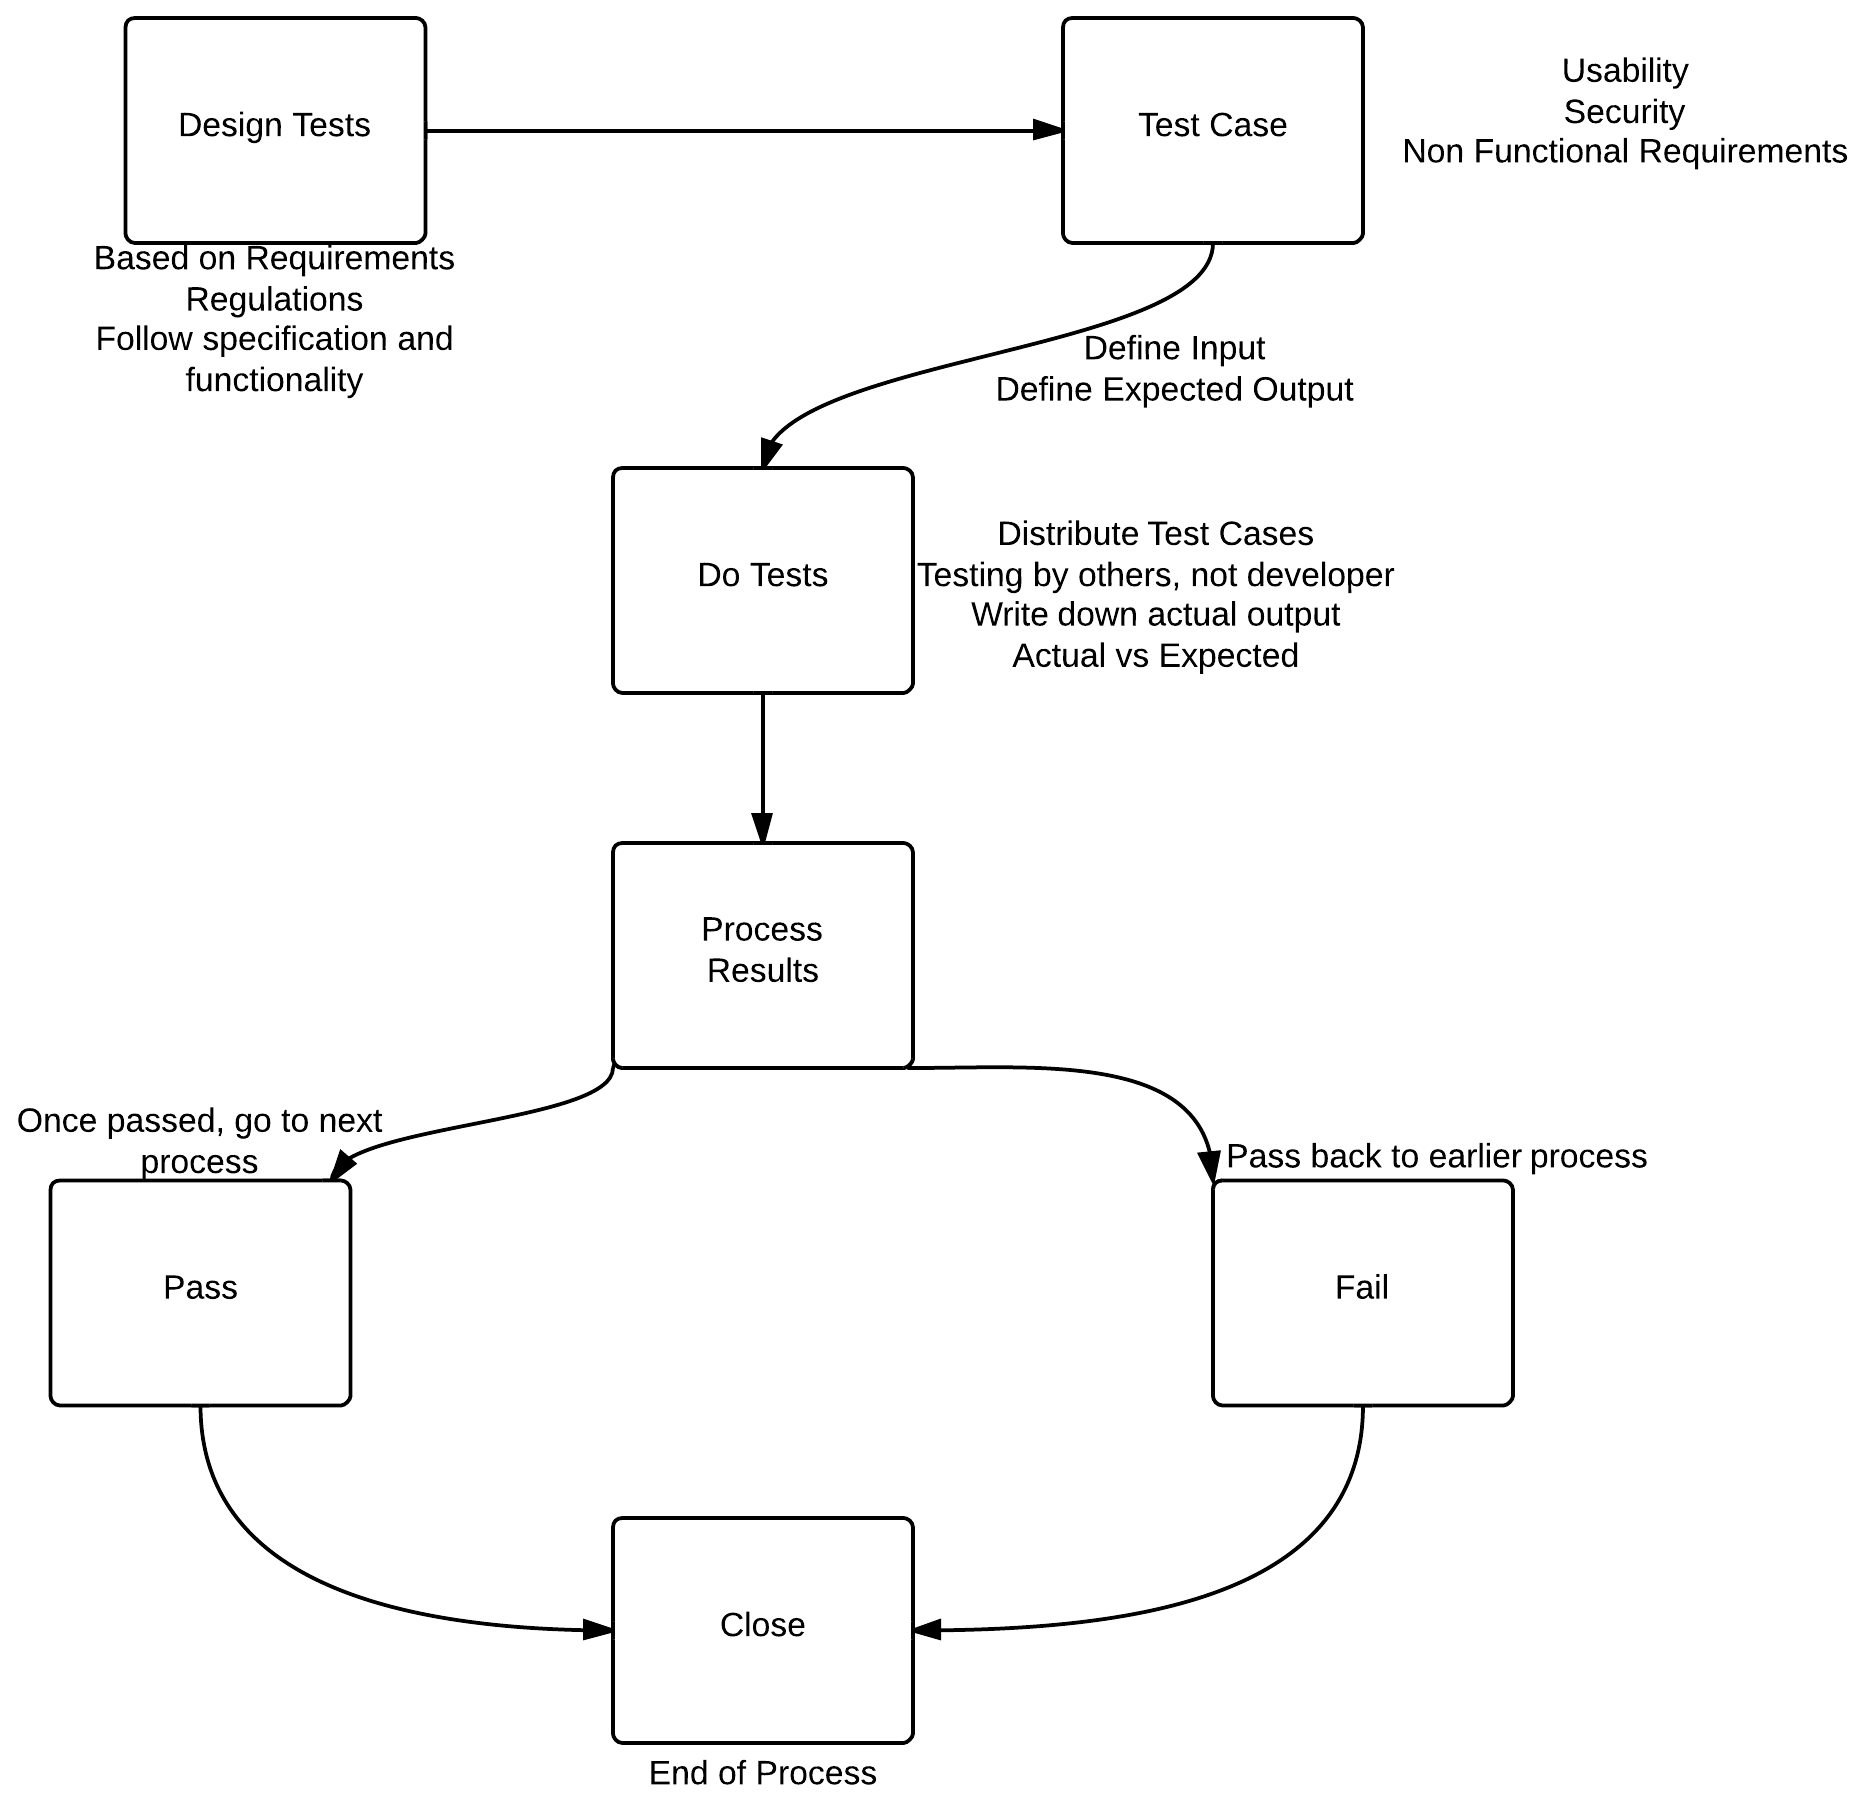
\includegraphics[scale=0.24]{testing.png}
\end{center}

\section{Paper}



\section{Meeting}

No meeting this week.

\chapter{Week 9}

\section{Learnings}

No lecture this week.

\section{Paper}

FYP!

\section{Meeting}

FYP!

\chapter{Week 10}

\section{Learnings}

FYP Demo Day. No lecture this week.

\section{Paper}

FYP!

\section{Meeting}

FYP!

\chapter{Week 11}

\section{Learnings}
\begin{enumerate}
\item Time to market for software very important
\begin{itemize}
\item Potential losses can be large due to competitor advantages, cost of development, lost earnings
\end{itemize}
\item Global Distance in Global Software Development
\begin{itemize}
\item Temporal Distance, Geographical Distance, Linguistic Distance and Cultural Distance all make up Global Distance. 
\end{itemize}
\item Social Capital
\begin{itemize}
\item Investment in people, and the relationships between them key to success of GSD. 
\end{itemize}
\item Local Process may not work as a Global Process
\begin{itemize}
\item Cognisance of different cultures and people important when defining a local process
\end{itemize}
\end{enumerate}

\section{Paper}

A concept that was mentioned this week was that of Transactive Memory Systems, and how an organisation utilises them, or should utilise them, to manage people leaving a team. A paper I looked through was "Transactive memory systems in organizations: Matching tasks, expertise, and people" \parencite{week11}. 

Transactive Memory "is the shared division of cognitive labour with respect to the encoding, storage, retrieval and communication of information from different knowledge bases" \parencite{week11}. Each member in a team contains their own knowledge, and this knowledge contributes to the overall success of a project. The project team then assigns tasks based on the perception of each others expertise. One of the key things needed for this type of system to work in an organisation is "cognitive interdependence" \parencite{week11}, or that the members of the group know that they need each other.

\section{Meeting}

No meeting this week. Informal agreement to meet next week to focus on paper and quality plan process.

\chapter{Week 12}

\section{Learnings}
\begin{enumerate}
\item
\begin{itemize}
\item
\end{itemize}
\item
\begin{itemize}
\item
\end{itemize}
\item
\begin{itemize}
\item
\end{itemize}
\end{enumerate}

\section{Paper}

\section{Meeting}


